\documentclass{article}
\usepackage[utf8]{inputenc}
\usepackage{graphicx}
\usepackage{enumitem}
\begin{document}
\section{Zalihe namirnica}
Pregled stanja zaliha namirnica je slučaj upotrebe u kome se formalizuje način na koji ugostiteljski objekat planira nabavku namirnica, nabavlja, a potom ih dodaje na stanje. U tom procesu učestvuju menadžer nabavke (zaposleni) i dobavljač. 

\begin{itemize}
\item Zaposleni kreira spisak namirnica čija je trenutna količina ispod propisane minimalne. Na osnovu tog spiska, kreira porudžbinu. Kasnije, nakon isporuke porudžbine, unosi u bazu pristiglu robu.
\item Dobavljač isporučuje ugostiteljskom objektu namirnice u traženoj količini.
\end{itemize}
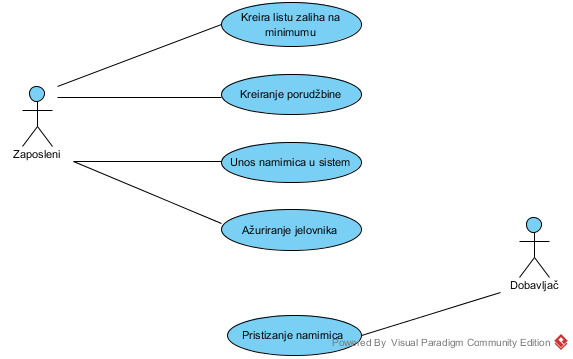
\includegraphics[width=\textwidth]{zalihe.png}
\subsection{\textbf{Use Case}: Zalihe na minimumu}
\textbf{Akter:} Radnik/menadžer nabavke\\
\textbf{Ulaz:} Nema\\
\textbf{Izlaz:} Kreiran je spisak namirnica čije su zalihe na minimumu.\\
\textbf{Preduslovi:} Radnik poseduje username i lozinku za prijavljivanje na glavni sistem gde se nalaze informacije o namirnicama.\\
\textbf{Postuslov:} Uspešno je kreiran spisak namirnica.\\
\textbf{Glavni tok:} 
\begin{enumerate}
	\item Radnik se prijavljuje na sistem.
	\item Radnik zahteva od sistema spisak namirnica za koje važi da je trenutna količina manja od minimalne propisane.
	\item Sistem generiše listu namirnica koje zadovoljavaju prethodno navedeni uslov.
\end{enumerate}
\textbf{Alternativni tok:} Ukoliko ne postoji ni jedan proizvod koji ima definisanu minimalnu količinu, izveštaj o zalihama na minimumu se ne može generisati.\\

\subsection{\textbf{Use Case}: Kreiranje porudžbine}
\textbf{Akter:} Radnik/menadžer nabavke\\
\textbf{Ulaz:} Lista namirnica čije su zalihe na minimumu.\\
\textbf{Izlaz:} Lista poručenih namirnica.\\
\textbf{Preduslovi:} Radnik ima uvid u spisak namirnica čija je količina manja od poželjne.\\
\textbf{Postuslov:} Porudžbina je kreirana.\\
\textbf{Glavni tok:} 
\begin{enumerate}
	\item Radnik uzima listu namirnica koje bi trebalo nabaviti.
	\item Za svaku namirnicu procenjuje količinu za nabavku. 
	\item Na spisak može dodati i namirnice kojih nema i nikada ih nije bilo u sistemu. 
	\item Kreira porudžbinu.
\end{enumerate}
\textbf{Alternativni tok:} Ukoliko je lista namirnica na minimalnim zalihama prazna, procena se ne vrši.\\

\subsection{\textbf{Use Case}:  Pristizanje namirnica}
\textbf{Akter:} Dobavljač\\
\textbf{Ulaz:} Lista poručenih namirnica.\\
\textbf{Izlaz:} Lista namirnica koje je dobavljač isporučio ugostiteljskom objektu.\\
\textbf{Preduslovi:} Dobavljač je dobio porudžbinu.\\
\textbf{Postuslov:} Namirnice su isporučene kupcu i kreirana je lista dostavljenih proizvoda.\\
\textbf{Glavni tok:} 
\begin{enumerate}
	\item Dobavljač je primio porudžbinu.
	\item Procenjuje da li je njegva firma u mogućnosti da odgovori na zahteve ugostiteljskog objekta, ukoliko nije, otkazuje porudžbinu.
	\item Za svaku namirnicu odlučuje da li će isporučiti u smanjenoj ili traženoj količini.
	\item Isporučuje robu ugostiteljskom objektu.
	\item Pri isporuci dostavljena je lista namirnica koje su isporučene.
\end{enumerate}
\textbf{Alternativni tok:} Zbog manjka raspoloživih namirnica, dobavljač otkazuje porudžbinu.\\

\subsection{\textbf{Use Case}: Unos namirnica u sistem}
\textbf{Akter:} Radnik\\
\textbf{Ulaz:} Spisak namirnica koje je dobavljač isporučio.\\
\textbf{Izlaz:} Ažurirana je lista namirnica.\\
\textbf{Preduslovi:} Radnik poseduje username i lozinku za prijavljivanje na glavni sistem. Dobavljač je dostavio poručene namirnice.\\
\textbf{Postuslov:} Ažurirane su količine namirnica i eventualno unete nove.\\
\textbf{Glavni tok:} 
\begin{enumerate}
	\item Radnik je dobio listu isporučenih namirnica.
	\item Radnik se prijavljuje na sistem.
	\item Za svaki od proizvoda sa liste, radnik ažurira proizvod u sistemu tako što dodaje pristiglu količinu.
	\item Ukoliko proizvod ne postoji u sistemu, radnik kreira novi.
	\item Ažurira novokreiranu namirnicu pristiglom količinom i eventualno definiše minimalnu količinu. 
\end{enumerate}
\textbf{Alternativni tok:} Porudžbina je otkazana od strane dobavljača, nema unosa.\\

\subsection{\textbf{Use Case}: Ažuriranje jelovnika}
\textbf{Akter:} Radnik\\
\textbf{Ulaz:} Spisak namirnica u restoranu i spisak jela sa neophodnim namirnicama za njihovu pripremu.\\
\textbf{Izlaz:} Kreiran je jelovnik.\\
\textbf{Preduslovi:} Radnik poseduje username i lozinku za prijavljivanje na glavni sistem. Spisak jela i sastojaka od kojih se pripremaju nije prazan.\\
\textbf{Postuslov:} Jelovnik je kreiran. Gosti i zaposleni ga mogu videti.\\
\textbf{Glavni tok:} 
\begin{enumerate}
	\item Radnik zahteva od sistema ažuriranje jelovnika.
	\item Sistem na njegov zahtev kreira novi jelovnik tako što iz liste jela izbacuje ona za čiju pripremu nedostaje makar jedan sastojak.
	\item Kreirani jelovnik postaje aktuelni jelovnik ugostiteljskog objekta.
\end{enumerate}
\textbf{Alternativni tok:} Ne postoje podaci koji povezuju jela i namirnice, novi jelovnik se ne može generisati. Aktuelni jelovnik se ne ažurira.\\
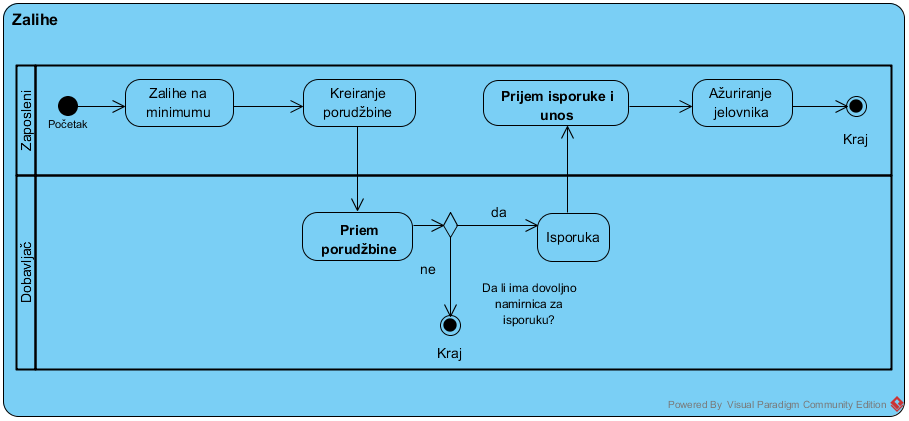
\includegraphics[width=\textwidth]{zalihe-activity.png}


\end{document}
